\documentclass[12pt,fleqn]{article}\usepackage{../common}
\begin{document}
Lineer Regresyon

Bir hedef degiskeninin bir veya daha fazla kaynak degiskenine olan
baglantisini bulmak icin en basit yontemlerden biri bu iliskinin lineer
oldugunu kabul etmektir, ve degiskenlerin carpildigi agirliklari bulmak
icin En Az Kareler (Least Squares) en iyi bilinen yontemlerden biri. En Az
Kareleri daha once pek cok degisik ders notlarinda, yazida turettik. Mesela
{\em Cok Degiskenli Calculus Ders 9}, {\em Lineer Cebir Ders 15}, ya da
Uygulamali Matematik yazilarindan {\em Regresyon, En Az Kareler (Least
  Squares)} yazilarinda bu turetimi gorduk. 

Lineer Regresyonun sadece iki degisken temelli islemek gerekirse, 

$$ Y = \beta_0 + \beta_1 x + \epsilon$$

olabilir. Burada $\epsilon$ $N(0,\sigma^2)$ dagilimindan gelen hatadir ve
$\sigma$ bilinmez. Eger veriyi $(x_1,y_1),...(x_n,y_n)$ ikili olarak
grafiklesek 

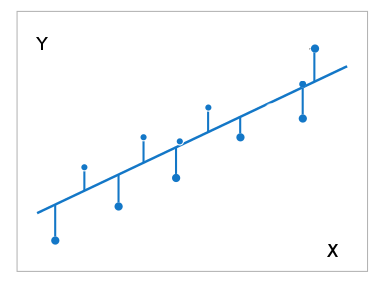
\includegraphics[height=4cm]{lin_01.png}

gibi gozukebilirdi, lineer regresyon ile yapmaya calistigimiz tum noktalara
olabilecek en yakin duz cizgiyi (ustte goruldugu gibi) bulmaktir. 

Bu duz cizgiyi (ki boyutlu ortamda bu cizgi bir hiper duzlem olurdu), En Az
Kareler bulduktan sonra bazi ``tahmini'' katsayi degerleri elde edecegiz,
katsayilar $\hat{\beta}_0,\hat{\beta}_1$ olarak tanimlanir. Kullandigimiz
noktasyon istatistikteki ``tahmin edici (estimator)'' notasyon ile uyumlu,
bunu bilerek yaptik. Ve bu tahmin ediciler ile elde edilen $y$'nin kendisi
de bir tahmin edici haline gelir ve bir duz cizgiyi tanimlar,

$$ \hat{y} = \hat{\beta}_0 + \hat{\beta}_1x $$


Satis ve Reklamlar

\begin{minted}[fontsize=\footnotesize]{python}
import pandas as pd
import statsmodels.formula.api as smf
df = pd.read_csv('adv.csv',usecols=[1,2,3,4])
print df[:2]
\end{minted}

\begin{verbatim}
      TV  Radio  Newspaper  Sales
0  230.1   37.8       69.2   22.1
1   44.5   39.3       45.1   10.4
\end{verbatim}

\begin{minted}[fontsize=\footnotesize]{python}
results = smf.ols('Sales ~ 1 + TV', data=df).fit()
print results.summary()
\end{minted}

\begin{verbatim}
                            OLS Regression Results                            
==============================================================================
Dep. Variable:                  Sales   R-squared:                       0.612
Model:                            OLS   Adj. R-squared:                  0.610
Method:                 Least Squares   F-statistic:                     312.1
Date:                Fri, 14 Mar 2014   Prob (F-statistic):           1.47e-42
Time:                        17:28:29   Log-Likelihood:                -519.05
No. Observations:                 200   AIC:                             1042.
Df Residuals:                     198   BIC:                             1049.
Df Model:                           1                                         
==============================================================================
                 coef    std err          t      P>|t|      [95.0% Conf. Int.]
------------------------------------------------------------------------------
Intercept      7.0326      0.458     15.360      0.000         6.130     7.935
TV             0.0475      0.003     17.668      0.000         0.042     0.053
==============================================================================
Omnibus:                        0.531   Durbin-Watson:                   1.935
Prob(Omnibus):                  0.767   Jarque-Bera (JB):                0.669
Skew:                          -0.089   Prob(JB):                        0.716
Kurtosis:                       2.779   Cond. No.                         338.
==============================================================================
\end{verbatim}

\begin{minted}[fontsize=\footnotesize]{python}
results = smf.ols('Sales ~ 1 + Radio', data=df).fit()
print results.summary()
\end{minted}

\begin{verbatim}
                            OLS Regression Results                            
==============================================================================
Dep. Variable:                  Sales   R-squared:                       0.332
Model:                            OLS   Adj. R-squared:                  0.329
Method:                 Least Squares   F-statistic:                     98.42
Date:                Fri, 14 Mar 2014   Prob (F-statistic):           4.35e-19
Time:                        17:41:33   Log-Likelihood:                -573.34
No. Observations:                 200   AIC:                             1151.
Df Residuals:                     198   BIC:                             1157.
Df Model:                           1                                         
==============================================================================
                 coef    std err          t      P>|t|      [95.0% Conf. Int.]
------------------------------------------------------------------------------
Intercept      9.3116      0.563     16.542      0.000         8.202    10.422
Radio          0.2025      0.020      9.921      0.000         0.162     0.243
==============================================================================
Omnibus:                       19.358   Durbin-Watson:                   1.946
Prob(Omnibus):                  0.000   Jarque-Bera (JB):               21.910
Skew:                          -0.764   Prob(JB):                     1.75e-05
Kurtosis:                       3.544   Cond. No.                         51.4
==============================================================================
\end{verbatim}

\begin{minted}[fontsize=\footnotesize]{python}
results = smf.ols('Sales ~ 1 + Newspaper', data=df).fit()
print results.summary()
\end{minted}

\begin{verbatim}
                            OLS Regression Results                            
==============================================================================
Dep. Variable:                  Sales   R-squared:                       0.052
Model:                            OLS   Adj. R-squared:                  0.047
Method:                 Least Squares   F-statistic:                     10.89
Date:                Fri, 14 Mar 2014   Prob (F-statistic):            0.00115
Time:                        17:42:20   Log-Likelihood:                -608.34
No. Observations:                 200   AIC:                             1221.
Df Residuals:                     198   BIC:                             1227.
Df Model:                           1                                         
==============================================================================
                 coef    std err          t      P>|t|      [95.0% Conf. Int.]
------------------------------------------------------------------------------
Intercept     12.3514      0.621     19.876      0.000        11.126    13.577
Newspaper      0.0547      0.017      3.300      0.001         0.022     0.087
==============================================================================
Omnibus:                        6.231   Durbin-Watson:                   1.983
Prob(Omnibus):                  0.044   Jarque-Bera (JB):                5.483
Skew:                           0.330   Prob(JB):                       0.0645
Kurtosis:                       2.527   Cond. No.                         64.7
==============================================================================
\end{verbatim}

\begin{minted}[fontsize=\footnotesize]{python}
results = smf.ols('Sales ~ 1 + TV + Radio + Newspaper ', data=df).fit()
print results.summary()
\end{minted}

\begin{verbatim}
                            OLS Regression Results                            
==============================================================================
Dep. Variable:                  Sales   R-squared:                       0.897
Model:                            OLS   Adj. R-squared:                  0.896
Method:                 Least Squares   F-statistic:                     570.3
Date:                Fri, 14 Mar 2014   Prob (F-statistic):           1.58e-96
Time:                        17:45:35   Log-Likelihood:                -386.18
No. Observations:                 200   AIC:                             780.4
Df Residuals:                     196   BIC:                             793.6
Df Model:                           3                                         
==============================================================================
                 coef    std err          t      P>|t|      [95.0% Conf. Int.]
------------------------------------------------------------------------------
Intercept      2.9389      0.312      9.422      0.000         2.324     3.554
TV             0.0458      0.001     32.809      0.000         0.043     0.049
Radio          0.1885      0.009     21.893      0.000         0.172     0.206
Newspaper     -0.0010      0.006     -0.177      0.860        -0.013     0.011
==============================================================================
Omnibus:                       60.414   Durbin-Watson:                   2.084
Prob(Omnibus):                  0.000   Jarque-Bera (JB):              151.241
Skew:                          -1.327   Prob(JB):                     1.44e-33
Kurtosis:                       6.332   Cond. No.                         454.
==============================================================================
\end{verbatim}


\begin{minted}[fontsize=\footnotesize]{python}
print df.corr()
\end{minted}

\begin{verbatim}
                 TV     Radio  Newspaper     Sales
TV         1.000000  0.054809   0.056648  0.782224
Radio      0.054809  1.000000   0.354104  0.576223
Newspaper  0.056648  0.354104   1.000000  0.228299
Sales      0.782224  0.576223   0.228299  1.000000
\end{verbatim}

Tek Tahmin Icin Guven Araligi

\begin{minted}[fontsize=\footnotesize]{python}
import pandas as pd
import statsmodels.formula.api as smf
df = pd.read_csv('cig.csv',sep='\t*')
results = smf.ols('mortality ~ consump', data=df).fit()
print results.summary()
print 'artik standart sapmasi (residual sd)', np.sqrt(results.mse_resid)
\end{minted}

\begin{verbatim}
                            OLS Regression Results                            
==============================================================================
Dep. Variable:              mortality   R-squared:                       0.532
Model:                            OLS   Adj. R-squared:                  0.508
Method:                 Least Squares   F-statistic:                     21.62
Date:                Mon, 21 Apr 2014   Prob (F-statistic):           0.000175
Time:                        16:21:44   Log-Likelihood:                -109.47
No. Observations:                  21   AIC:                             222.9
Df Residuals:                      19   BIC:                             225.0
Df Model:                           1                                         
==============================================================================
                 coef    std err          t      P>|t|      [95.0% Conf. Int.]
------------------------------------------------------------------------------
Intercept     15.7711     29.579      0.533      0.600       -46.138    77.680
consump        0.0601      0.013      4.649      0.000         0.033     0.087
==============================================================================
Omnibus:                        0.278   Durbin-Watson:                   2.671
Prob(Omnibus):                  0.870   Jarque-Bera (JB):                0.389
Skew:                          -0.227   Prob(JB):                        0.823
Kurtosis:                       2.513   Cond. No.                     6.64e+03
==============================================================================

Warnings:
[1] The condition number is large, 6.64e+03. This might indicate that there are
strong multicollinearity or other numerical problems.
artik standart sapmasi (residual sd) 46.7082590622
\end{verbatim}

\begin{minted}[fontsize=\footnotesize]{python}
pred = results.predict(pd.Series({ 'consump': 4200,}))[0]
print pred
\end{minted}

\begin{verbatim}
268.181363084
\end{verbatim}

\begin{minted}[fontsize=\footnotesize]{python}
from scipy.stats.distributions import t
s = np.sqrt(results.mse_resid)
print 's',s,'n',n
n = len(df)
xnew = 4200
xbar = df['consump'].mean()
xvar = df['consump'] - df['consump'].mean()
xvar = np.sum(xvar*xvar)
print 'xbar',xbar, 'xvar',xvar
print (xnew-xbar)**2
w = -t.ppf(0.025,n-2) * s * np.sqrt( 1/float(n) + ((xnew-xbar)**2) / xvar )
print 'w',w
print '(', pred - w, pred + w, ')'
\end{minted}

\begin{verbatim}
s 46.7082590622 n 21
xbar 2148.0952381 xvar 13056523.8095
4210313.15193
w 59.4730120398
( 208.708351045 327.654375124 )
\end{verbatim}


Kaynaklar

[1] Introduction to Mathematical Statistics and Its Applications, sf. 569

[2] Runger et al, Applied Statistics and Probability for Engineers, sf. 393





\end{document}


